\section{Theoretical background}
In this chapter, we will explain all the relevant background information needed to follow along with the thesis. \\
We will start by defining the main tasks and continue with describing all the used machine learning techniques. The last section will be about metrics for evaluation.

\subsection{Tasks}
We are going to evaluate our approaches on the two following tasks.

\subsubsection{Validity Classification}
As described in \cite{argsvalidnovel2022}, a conclusion of a premise is considered valid if it follows naturally from its premise. \\
Following this definition, validity classification is a binary classification task in which we want to determine whether a conclusion is valid, given its premise. The label $1$ corresponds to a valid conclusion and the label $0$ to an invalid conclusion \cite{argsvalidnovel2022}.

\subsubsection{Stance Classification}
Our second main tasks is called stance classification. It is a classification task in which we want to decide whether the author of a text is for, against or neutral towards a certain statement \cite{mohammad2017stance}.

\subsection{Language Models}
A language model (LM) is a model that assigns probabilities to sequences of words \cite{languagemodels2023}. \\
In this thesis, we will focus on masked LMs. These models are able to predict a masked word from a sentence, e.g.
\begin{center}
	\textit{Berlin is the capital of} \textbf{[MASK]}.
\end{center}
The model will then return a set of words and their corresponding probabilities to fill this [MASK] token \cite{bert}. LMs are often times pre-trained on large unlabeled text corpora to generate language representations like word vector embeddings which can later be fine-tuned on more specific tasks. In the next sections, we will present a few of these models.

\subsubsection{BERT}
BERT (Bidirectional Encoder Representations from Transformers) is a large LM (LLM) proposed by Delvin et al. \cite{bert}. Unlike older language models based on LSTMs which can only predict the next token based on the previous tokens, BERT uses a bidirectional approach. This is done by using the aforementioned masked LM pre-training objective. In this approach, a part of the input words gets masked and the training objective is to predict the original word based on its left and right context. Together with the next sentence prediction objective, this completes the pre-training for BERT. This model can now be used to solve many downstream tasks like classification or question answering, just by adding another layer on top. \\
We will primarily use BERT for masked language modeling and directly for validity and stance classification. \\

\textbf{Model Architecture} \\
Although we do not need to understand BERT in every detail, one important part is needed in the course of this thesis, namely how the input and output is represented. \\
Most importantly, for every input sequence, a special [CLS] token will be added as first character. This token is used in the last hidden state as an aggregate representation for the entire sequence. It can then be used for further downstream tasks like classification. The vector representations for all the other tokens in the output sequence are only used for token-level tasks like part-of-speech-tagging. Furthermore, a [SEP] token is added after each input sequence. With this technique, we can input two sequences as one into BERT which is used to perform the next sentence prediction task in the pre-training.


\subsubsection{RoBERTa}
RoBERTa is a LLM based on BERT \cite{roberta}. It improves BERT by
\begin{enumerate}
	\item longer training with more data,
	\item removing the next sentence prediction objective,
	\item training on longer sequences,
	\item dynamically changing the masking pattern.
\end{enumerate}

\subsection{Gradient-Boosted Trees}
Gradient-Boosted Trees are a form of random forests. Both combine multiple decision trees to produce one classifier but they differ in building the individual trees and in combining them \cite{gradboost}. A decision tree splits the data at each node until the leaf nodes are reached. These leaf nodes nodes then correspond to a certain label. In gradient boosting, decision trees with only a few splits are constructed. These trees are then added together sequentially while minimizing a loss function when adding each tree.

\subsubsection{XGBoost and LightGBM}
XGBoost and LightGBM are both gradient boosting frameworks using decision trees which significantly improve the performance and training speed of standard gradient boosting algorithms \cite{xgboost, lgbm}.

\subsection{Evaluation Metrics}
To evaluate our models, we need to define evaluation metrics. There are many different established metrics to use. In this section we will give an overview of the ones we are going to use along this thesis. These definitions are adapted from Hossin and Sulaiman \cite{metrics}.

\subsubsection{Binary Classification Metrics}

\textbf{Confusion Matrix} \\ \\
For binary classification, one can represent the results in a so called \textit{confusion matrix}. The rows of this matrix represent the predicted classes and the columns represent the true classes. The values in the matrix correspond to the four possible outcomes:
\begin{itemize}
	\item[\textbullet] True Positive (TP): Correctly classified positive instances
	\item[\textbullet] True Negative (TN): Correctly classified negative instances
	\item[\textbullet] False Positive (FP): Wrongly classified negative instances
	\item[\textbullet] False Negative (FN): Wrongly classified positive instances
\end{itemize}
An example of the final matrix is shown in Figure \ref{fig:confusion-matrix}.
\begin{figure}[h]
  \centering
  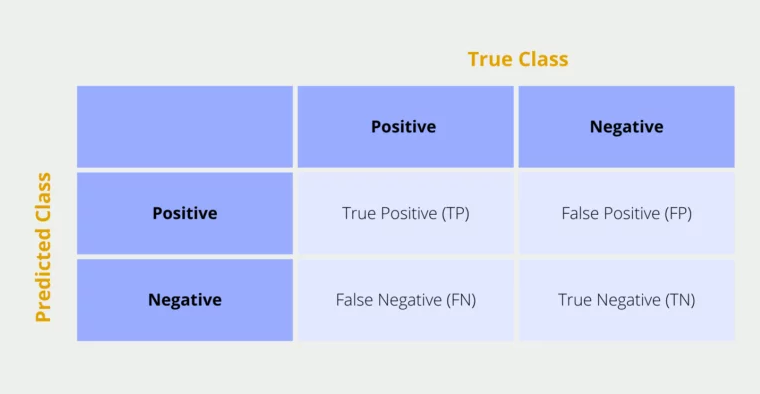
\includegraphics[width=8cm]{fig/confusion_matrix.png}
  \caption{Confusion Matrix \cite{confusion}.}%
  \label{fig:confusion-matrix}
\end{figure}

\textbf{Recall} \\ \\
Recall measures the fraction of positive instances that are correctly classified.

\begin{equation}
	R = \frac{TP}{TP + FN}
\end{equation}

\textbf{Precision} \\ \\
Precision measures the correctly classified positive instances in relation to the overall number of positively predicted instances

\begin{equation}
	P = \frac{TP}{TP + FP}
\end{equation}

\textbf{F1-Score} \\ \\
The F1 score is the harmonic mean between recall and precision.

\begin{equation}
	\text{F1} = \frac{2 \cdot P \cdot R}{P + R}
\end{equation}

\subsubsection{Multi-Class Metrics}
In the case of stance classification, we have three classes instead of two. Therefore we have to adept the calculation of these evaluation metrics for the non-binary case. In the following definitions, let $C$ be the number of classes. \\

\textbf{Averaged Recall} \\ \\
Macro average of the per-class recall.

\begin{equation}
	R_M = \frac{\sum\limits_{i=1}^{C} \frac{TP_i}{TP_i + FN_i}}{C}
\end{equation}

\textbf{Averaged Precision} \\ \\
Macro average of the per-class precision.

\begin{equation}
	P_M = \frac{\sum\limits_{i=1}^{C} \frac{TP_i}{TP_i + FP_i}}{C}
\end{equation}

\textbf{Averaged F1-Score} \\ \\
The average of the per-class F1-Score.

\begin{equation}
	\text{F1} = \frac{2 \cdot P_M \cdot R_M}{P_M + R_M}
\end{equation}
